% !TEX root = trkjet.tex

The analysis procedure uses similar cuts and corrections as in \cite{PhysRevC.98.024908} with the additional requirement of being done differentially in \rvar. Reconstructed tracks are associated with a reconstructed jet if they fall within $\Delta R < 0.8$ of the jet axis and are constructed as:

\begin{eqnarray}
\dfrac{\fd^{2} \nchmeas }{ \fd \pttrk \fd r} = \frac{1}{\varepsilon(\pttrk,\etatrk)} \frac{\Delta \Nch(\pttrk,\ptjet,r)}{\Delta\pttrk \Delta r}
\end{eqnarray}

where $\Delta \Nch (\pttrk,r)$ represents the number of associated tracks within a given \pttrk\ and $r$ range. The efficiency correction is applied as a $1/\varepsilon(\pttrk,\etatrk)$ weight on a track-by-track basis, assuming $\pttrk = \pTtrue$. While that assumption is not strictly valid, the efficiency varies sufficiently slowly with $\pTtrue$ that the error
introduced by this assumption is less than 1\%. The efficiency increases from about 80\% at \mbox{$ \pt = 1.0$ \GeV} to about 90\% at $ \pt = 10 $ \GeV, and is approximately constant thereafter. The variation of of the efficiency as a function of \ptjet\ for the charged-particle transverse momentum range under investigation is less than 3\%. In \pbpb\ collisions, the centrality dependence to the efficiency is also at the level of 3\%.

The measured track yields in \pp\ and \PbPb\ collisions need to be corrected for the presence of fake tracks and contributions from charged particles from the UE in \pbpb\ collisions. The UE contribution is evaluated as a function of \pttrk, \ptjet, $r$, azimuthal distance to the second order reaction plane angle~($\Psi_{2}$)~\cite{ATLAS:2012at}, and the collision centrality. The UE charged-particle yields $\fd \nchUE/ \fd \pttrk$, are evaluated over \mbox{$1.0 < \pttrk < 10$~\GeV}. MC studies show that the UE contribution is negligible for charged particles with $\pttrk>10$~GeV.

The UE contribution is estimated using the \PbPb\ MC overlay events where the efficiency corrected differential yields of charged particles without a truth match, $\mathrm{d}N^{4}_{\mathrm{ch}}/\mathrm{d}\phi\mathrm{d}\eta\mathrm{d}\pttrk\mathrm{d}\Psi_{2}$ are evaluated separately for
each centrality selection. Here $\fd \Psi_{2}$ denotes the azimuthal distance between the charged particle and the second-order reaction plane angle\footnote{The reaction plane angle $\Psi$ is determined on an event-by-event basis by a standard method using the $\phi$ variation of transverse energy in the forward calorimeter}. 
%Charged particles associated with a reconstructed jet with $\ptjet > 90$~\GeV\ are assumed to originate in the hard process and are excluded from the estimation. 
These yields are further used to estimate the average, area normalized yields of charged particles for the jet under study, \mbox{$1/A(r) \times \fd^2 \nchUE(r) / \fd \pttrk \fd r|_{\mathrm{cent}}$} (``cent'' refers to centrality), where $A(r)$ is the area of the annulus at distance \rvar. The jet $\eta$ and $\phi$ positions, as well as the azimuthal distance of the jet to the second-order reaction plane angle are taken into account. The yields are independent of the angular distance $r$, decrease with the decreasing collision centrality, increasing \pttrk, and increasing azimuthal distance to the second-order reaction plane. The difference in the centrality distribution between overlay sample and the jet-triggered sample is accounted for by a reweighing procedure.

%The UE contribution is further corrected for the correlation between the actual UE yield underneath the jet and the jet energy resolution 
% discussed in Ref.~\cite{Aad:2014wha}. This effect is corrected by multiplicative correction factors, depending on \pTtrk, \ptjet, and collision centrality. The correction is estimated as a ratio of the UE evaluated by two different methods using the \PbPb\ MC samples. The first estimate is done by the 
% MB method discussed above.

A second method to calculate the UE is used to provide a systematic uncertainty. This method is adapted from the underlying event estimation method used in \cite{PhysRevC.98.024908} and uses a regular grid of 9 cones of size $R = 0.8$ to cover the full inner detector region. Cones within a distance of $dR=1.6$ to a reconstructed jet are excluded if $\ptjet > 90$ GeV or if they contain a track with $\pt > 10$ GeV. This exclusion removes biases from any hard processes. The resulting UE charged particle yields $\fd \nchUE^{\mathrm{Cone}}/ \fd \pTch$ are evaluated over the 1 -- 10 GeV range as a function of \pt, \ptjet, centrality, and \rvar, and are subsequently averaged over all cones according to
 \begin{eqnarray}
 \label{eq:Dptsub}
\frac{\fd n_{\mathrm{ch}}^{\mathrm{UE Cone}}}{\fd \pTch}  = \frac{1}{N_{\mathrm{cones}}} \frac{1}{\varepsilon} \frac{\Delta N^{\mathrm{cone}}_{\mathrm{ch}} (\pTch, \ptjet, \etajet)}{\Delta \pTch}
 \end{eqnarray}
 Here $N_{\mathrm{cones}}$ is the number of background cones associated with a given jet with \ptjet. $\Delta N^{\mathrm{cone}}_{\mathrm{ch}}$ is the number of charged particles summed across all background cones associated to the jet in question, and $\varepsilon$ is the efficiency for reconstructing a charged particle with $\pt^{\mathrm{ch}}$. The cone method estimates the UE yields only from events containing jets included in the analysis, ensuring that the background automatically had the correct distribution of centralities within a given centrality bin. The UE contribution as measured using the cone method in data needs three corrections:
 \subparagraph{Correction for $\eta$-dependence: } This accounts for differences in the yields of UE particles at the position of the jet and at the position of the track for the random cone entering the UE estimate. The correction is derived using the $\eta$ distribution of charged particles from MC overlay events.
 \subparagraph{Correction for flow: }  There is a correction applied to account for the difference in the azimuthal particle density due to elliptic flow. This correction is based on a parametrization of the \pTch and centrality dependence of previously measured elliptic flow coefficients, $v_{2}$ \cite{2019108}.  
\subparagraph{UE and Jet Energy Resolution correlation: } The steeply falling jet spectra coupled with the smearing due to a finite jet energy resolution leads to a net migration of jets from lower \pt\ to higher \pt\ values, causing the underlying event underneath a jet to be larger than what is estimated. This is accounted for by correcting the measured underlying event in data by a ratio of the underlying event measured by the nominal method in MC (which by definition considers only tracks without a truth match) and the cone method in MC. The size of the correction is negligible for larger $r$ values or low \pttrk\ where the UE is the largest and increases with decreasing $r$ values and increasing \pttrk. It has only a small dependence on \ptjet. 

The measured distributions both in \pp\ and \PbPb\ collisions are further corrected for the presence of fake tracks. The contribution from these tracks to the \Dptr\ distributions
is estimated from the MC samples without MB interactions overlaid. 
%The fraction of fake tracks is found to be below 2\% of the tracks that pass the selection in all track and jet kinematic regions in this analysis.
The corrected UE distributions with the addition of the fake track contribution, $1/A(r) \times \fd^2 \cnchUE (r) / \fd \pttrk \fd r |_{\mathrm{cent}}$, are then subtracted from the measured distributions.


\begin{figure}
\centerline{
 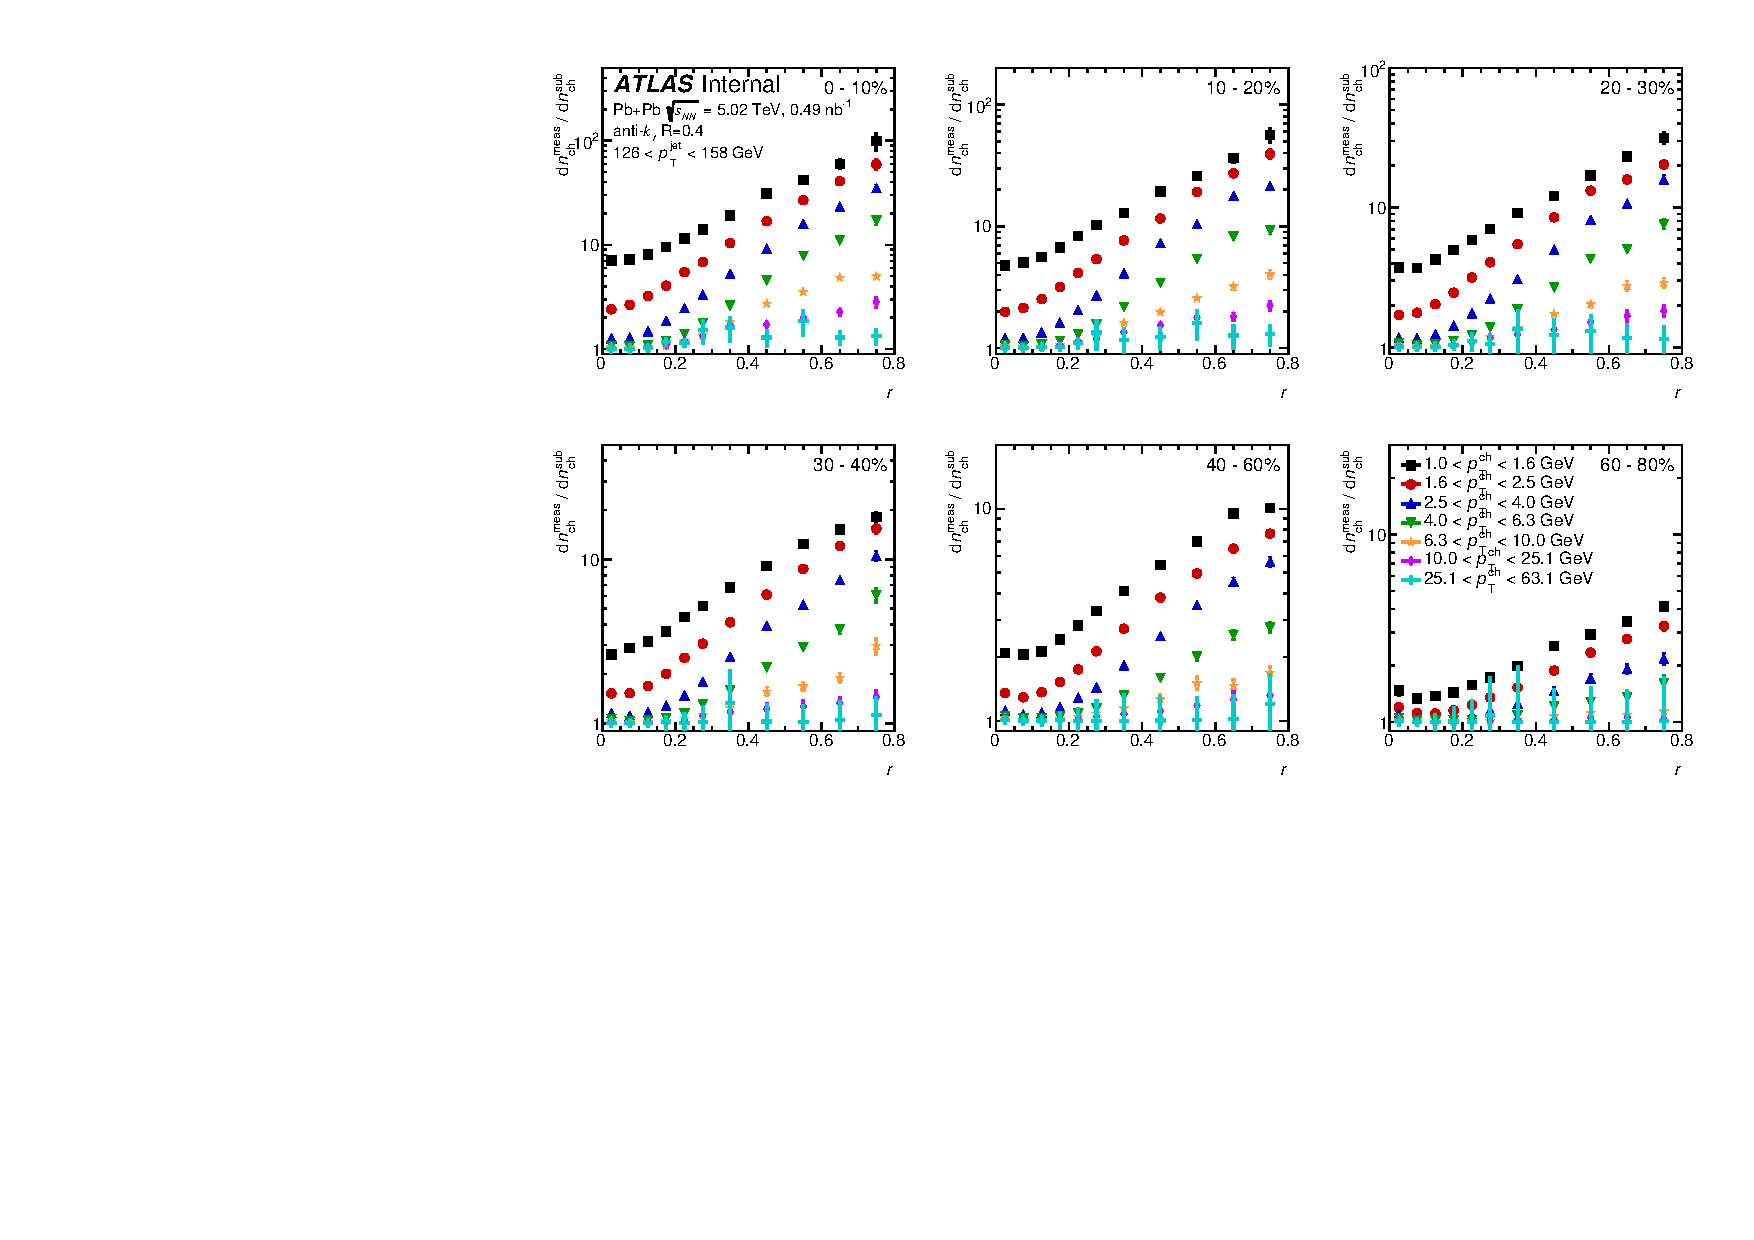
\includegraphics[width=0.95\textwidth]{figures/performance/UE_B2S_single_0.pdf}
}
\caption{
Ratio of the raw charged particle distributions to those after the subtraction of the UE
   and fake tracks as a function of \rvar\ for different \pttrk\ intervals, six centrality selections and for \ptjet\ between 126--158~\GeV.    
  }
\label{fig:UEsize}
\end{figure}

Figure~\ref{fig:UEsize} shows the charged-particle distributions prior to the UE and fake track subtraction, $ \fd^2 \nchmeas / \fd \pttrk \fd r$, divided by the distributions after the subtraction, $ \fd^2 \nchsub / \fd \pttrk \fd r $ as a function of \rvar\ for different \pttrk\ intervals and for six centrality selections, for jets in the 126--158 \GeV\  \ptjet\ range. The UE is the highest for 1.0~\GeV\ charged particles at large values of \rvar\ and in central collisions for \ptjet\ between 126--158~\GeV. It is rapidly decreasing towards more peripheral collisions, larger \pttrk\ and smaller \rvar.
Furthermore, the ratio is slowly decreasing with increasing \ptjet.

To remove the effects of the bin migration due to the jet energy and track-momentum resolution, the subtracted $1/A(r) \times \fd^2 \nchsub /\fd\pttrk \fd r$ distributions are corrected by a two-dimensional Bayesian unfolding~\cite{DAgostini:1994zf}
in \pttrk\ and \ptjet\ as implemented in the RooUnfold package~\cite{Adye:2011gm}.  
Two-dimensional unfolding is used because the calorimetric jet energy response depends on the fragmentation pattern of the jet~\cite{Aad:2011he}.
Four-dimensional response matrices are created from the MC samples using the generator-level and reconstructed \ptjet, and the generator-level and reconstructed charged-particle \pttrk. Separate unfolding matrices are constructed for the \pp\ and \PbPb\ system. The Bayesian procedure requires a choice in the number of iterations.
Additional iterations reduce the sensitivity to the choice of prior, but may
amplify statistical fluctuations in the distributions.
After four iterations the 
\Dptr\ distributions are found to be stable for both the \PbPb\ and \pp\ data. 
A separate one-dimensional Bayesian unfolding is used to correct the measured \ptjet\ spectra that are used to normalize the unfolded \Dptr\ distributions, $1/A(r) \times \fd^2 \nchunf / \fd \pt \fd r $. This uses the same number of iterations as in the case of the two-dimensional unfolding. To achieve better correspondence with the data, the response matrices for both the one and two dimensional unfolding are reweighed so that the distributions match the shapes in the reconstructed data.

Finally, an independent bin-by-bin unfolding procedure is used to correct for biases originating from the finite jet and track angular resolutions. Two corresponding \Dptr\ distributions are evaluated in MC samples, one using generator-level jets and primary particles and the other using simulated jets and charged particles with their reconstructed \pttrk\ replaced by generator-level transverse momentum, \pTtrue. The ratio of these two MC distributions provides a correction factor which is then applied to the data. 

%The final, particle-level corrected distributions are defined as:
%\begin{eqnarray}
% \label{eq:Dpt}
%   \Dptr = \frac{1}{N_\mathrm{jet}^\mathrm{unfolded}} \frac{1}{A(r)} \frac{\fd^2 \nchunf(r)}{\fd \pt \fd r},
% \end{eqnarray}
%where $\text{N}_{\text{jet}}^{\text{unfolded}}$ is the unfolded number of jets in a given \ptjet\ interval.

The performance of the full analysis procedure is validated in MC events where the entire correction procedure is performed using reconstructed jets and tracks, and the results are compared to the generator-level distributions. Large non-closure is observed for particles that are near the edge of the R = 0.4 jet cone and carry a significant fraction of the jet momentum. This effect is identified as an intrinsic property of the \antikt\ algorithm that tends to locate the jet axis in such a position that objects at distance \rvar\ from it are rare and soft. To be conservative, the analysis is restricted to the phase space where the non-closure is less than 5\%.

%The deviations from the exact recovery of the truth MC distributions, the non-closure, are included in the systematic uncertainties.
